% Context-size probing: Nunito, token chips, palette and horizontal bars
% adapted from the multibit watermark poster and the existing blog figure.
% Build with lualatex, then pdftoppm -r 144 -png -singlefile.
\documentclass[border=8bp]{standalone}
\usepackage{fontspec}
\setmainfont{Nunito}[Extension=.otf,UprightFont=*-Regular,BoldFont=*-Bold,
  ItalicFont=*-Italic,BoldItalicFont=*-BoldItalic,FontFace={sb}{n}{*-SemiBold},Numbers=Lining,WordSpace=1.12]
\setmonofont{DejaVuSansMono}[Extension=.ttf,BoldFont=*-Bold]
\usepackage{amsmath,xcolor,tikz,xfp}
\usetikzlibrary{calc,arrows.meta,decorations.pathreplacing}
\newlength\U \setlength\U{0.75bp}
\newcommand\fs[1]{\fontsize{\fpeval{#1*.75}bp}{\fpeval{#1*.75*1.22}bp}\selectfont\spaceskip=\fontdimen2\font\relax}
\newcommand\sbseries{\fontseries{sb}\selectfont}
\definecolor{wpink}{HTML}{C76DAC}
\definecolor{wpurple}{HTML}{8E7CC3}
\definecolor{ink}{HTML}{1F1F1F}
\definecolor{muted}{HTML}{5A5A5A}
\definecolor{panel}{HTML}{F2F2F2}
\definecolor{lpink}{HTML}{F6DDEE}
\definecolor{lpurple}{HTML}{E4DDF3}
\definecolor{dark}{HTML}{1C2B33}
\colorlet{dpink}{wpink!80!black}
\colorlet{dpurple}{wpurple!78!black}
\tikzset{
 tok/.style={rounded corners=5\U,minimum width=57\U,minimum height=55\U,inner sep=0,font=\fs{31}\ttfamily,text=ink,fill=panel},
 ctxtok/.style={tok,fill=lpurple},
 changed/.style={fill=lpink,draw=wpink,line width=2.4\U},
 arr/.style={-{Stealth[length=10bp]},line width=2.7\U,draw=ink}}
% #1 row y; #2 changed token's distance before choice (0 = reference).
\newcommand\sequence[2]{%
 \foreach \token [count=\j from 0] in {a,b,c,d,e,f} {
  \ifnum\j<2 \node[tok] at ({325+\j*68},#1) {\token};
  \else \node[ctxtok] at ({325+\j*68},#1) {\token}; \fi}
 \ifnum#2=5 \node[tok,changed] at (393,#1) {x}; \fi
 \ifnum#2=4 \node[ctxtok,changed] at (461,#1) {x}; \fi
 \node[tok,fill=white,draw=ink,line width=1.8\U,minimum width=120\U,font=\fs{27}\ttfamily] at (795,#1) {choice};
 \draw[arr] (709,#1) -- (727,#1);
 \draw[wpurple,line width=2\U] (431,{#1+39}) -- (431,{#1+49}) -- (695,{#1+49}) -- (695,{#1+39});}
% Schematic probabilities, each triple sums to 100%.
\newcommand\distribution[5]{%
 \foreach \word/\value [count=\j from 0] in {apple/#2,pear/#3,plum/#4} {
  \node[anchor=east,inner sep=0,font=\fs{25}\ttfamily,text=muted] at (999,{#1-37+\j*37}) {\word};
  \fill[panel] (1016,{#1-48+\j*37}) rectangle (1232,{#1-26+\j*37});
  \fill[#5] (1016,{#1-48+\j*37}) rectangle ({1016+3.6*\value},{#1-26+\j*37});
  \node[anchor=west,inner sep=0,font=\fs{25},text=ink] at (1248,{#1-37+\j*37}) {\value\%};}}
\begin{document}
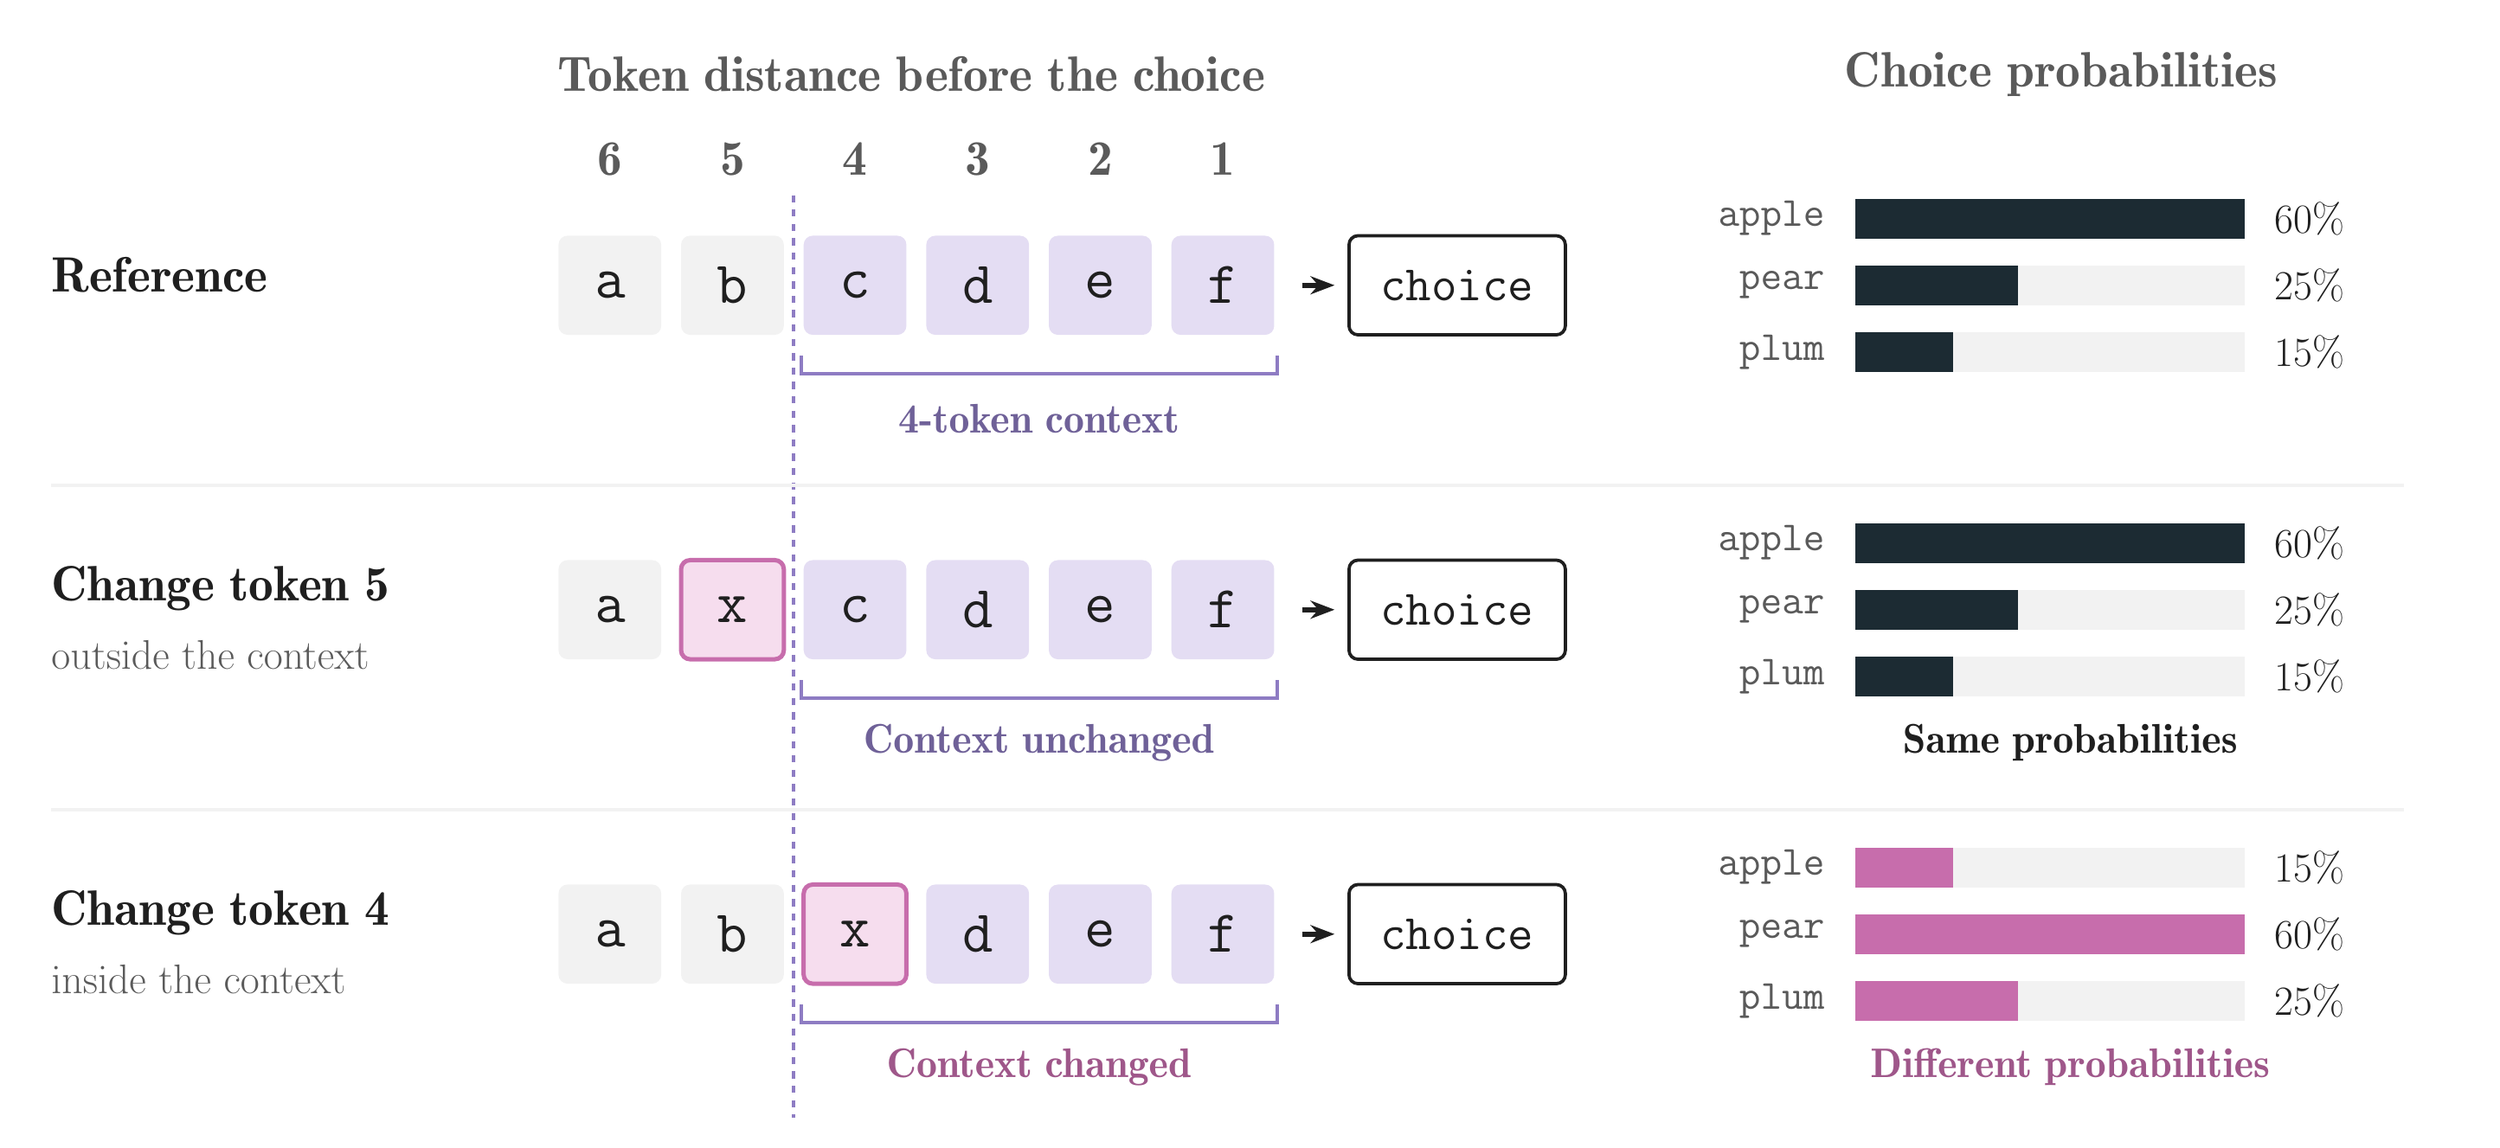
\begin{tikzpicture}[x=.75bp,y=-.75bp]
\path[use as bounding box] (0,0) rectangle (1360,610);
\node[anchor=west,inner sep=0,font=\fs{27}\sbseries,text=muted] at (296,28) {Token distance before the choice};
\foreach \i [count=\j from 0] in {6,5,4,3,2,1}
 \node[font=\fs{26}\sbseries,text=muted] at ({325+\j*68},75) {\i};
\node[font=\fs{28}\sbseries,text=muted] at (1130,28) {Choice probabilities};
\draw[wpurple,line width=2\U,dashed] (427,95) -- (427,607);
\node[anchor=west,inner sep=0,font=\fs{30}\sbseries,text=ink] at (15,139) {Reference};
\sequence{145}{0}
\distribution{145}{60}{25}{15}{dark}
\node[font=\fs{25}\sbseries,text=dpurple] at (563,219) {4-token context};
\draw[panel,line width=2\U] (15,256) -- (1320,256);
\node[anchor=west,inner sep=0,font=\fs{29}\sbseries,text=ink] at (15,313) {Change token 5};
\node[anchor=west,inner sep=0,font=\fs{25},text=muted] at (15,350) {outside the context};
\sequence{325}{5}
\distribution{325}{60}{25}{15}{dark}
\node[font=\fs{25}\sbseries,text=dpurple] at (563,399) {Context unchanged};
\node[font=\fs{25}\sbseries,text=ink] at (1135,399) {Same probabilities};
\draw[panel,line width=2\U] (15,436) -- (1320,436);
\node[anchor=west,inner sep=0,font=\fs{29}\sbseries,text=ink] at (15,493) {Change token 4};
\node[anchor=west,inner sep=0,font=\fs{25},text=muted] at (15,530) {inside the context};
\sequence{505}{4}
\distribution{505}{15}{60}{25}{wpink}
\node[font=\fs{25}\sbseries,text=dpink] at (563,579) {Context changed};
\node[font=\fs{25}\sbseries,text=dpink] at (1135,579) {Different probabilities};
\end{tikzpicture}
\end{document}
